\chapter{АППАРАТНАЯ ЧАСТЬ}
\section{Введение}

В данной работе объединительной платой назовем группу электрических разъемов соединенных друг с другом, напрямую или посредством специальных  электрических цепей, использующихся в качестве основы, чтобы соединить несколько печатных плат вместе и составить полную систему. Полная схема объединительной платы представлена в приложении А. Далее в этой главе рассмотрим специальные соединительные электрические цепи.

\section{Датчик угла поворота}

При снятии с датчика угла поворота (энкодера) сигналов во время переключения барабана наблюдается дребезг контактов, так как обработка сигнала контроллером ведется по прерыванию фронта канала А энкодера, необходимо создать надежную защиту от появления шумовых фронтов. Для исключения возможности попадания дребезга были использованы цепочка фильтра нижних частот и триггер Шмидта (SN54AC14FK), имеющих гистерезис как функцию преобразования сигнала (см. рис. \ref{fig:EndCSchm}).
\begin{figure}[ht]
	\centering
     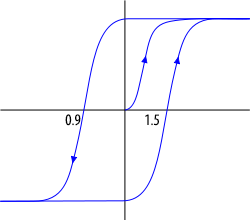
\includegraphics[scale=1.3]{Hysteresis.PNG}
	\caption{Петля гистерезиса SN54AC14FK.}
	\label{fig:Hysteresis}
\end{figure}

\begin{figure}[ht]
	\centering
     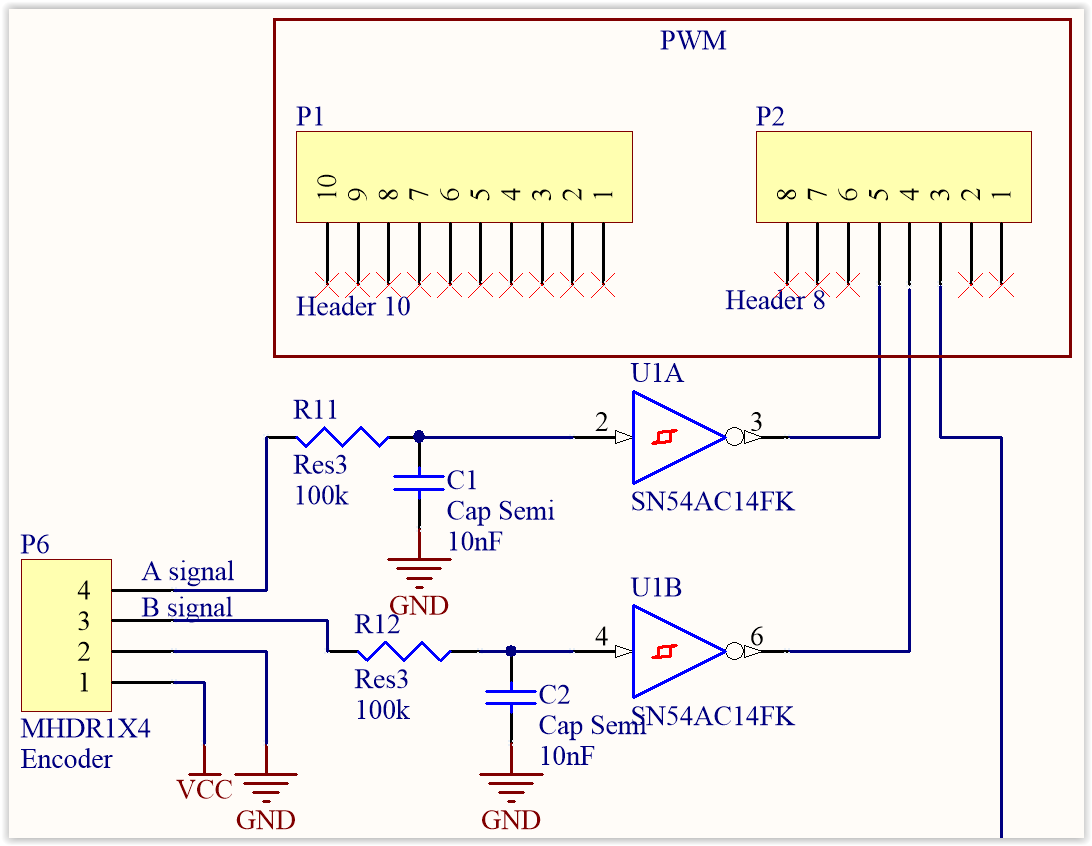
\includegraphics[scale=0.45]{endcoder_schm.PNG}
	\caption{Специальная соединительная схема датчика угла поворота.}
	\label{fig:EndCSchm}
\end{figure}
Дребезг может длиться порядка 10 мс, время за которое конденсатор зарядится на 99\% $ \tau=3*C*R=3 $ мс, триггер Шмидта имеет толщину гистерезисной петли от 0,4 до 1,5 вольта(см. рис. \ref{fig:Hysteresis}). 

\section{VGA}

Видеоадаптер VGA, в отличие от предыдущих видеоадаптеров, использует аналоговый сигнал для передачи цветовой информации. Переход на аналоговый сигнал был обусловлен необходимостью сокращения числа проводов в кабеле. 

Stimmer, автор открытой библиотеки кодов DueVGA, использовал изящное решения задачи подключения к контроллеру VGA интерфейса - программный делитель напряжения. Его механизм заключается в том, что к выходу подключёны  резисторы разного номинала, на которые подается напряжения 0 или 5 вольт, в зависимости от того на какие резисторы и какое напряжение (0 или 5) подается, на выходе мы получаем разное напряжение и, как итог, разные цвета отображаемого изображения. Развертка строк и фреймов задается сигналами Hsync и Vsync. Специальная соединительная схема VGA-контроллер содержит соединенные группы резисторов реализующие это решение(см. рис. \ref{fig:VGASchm}).
\begin{figure}[ht]
	\centering
     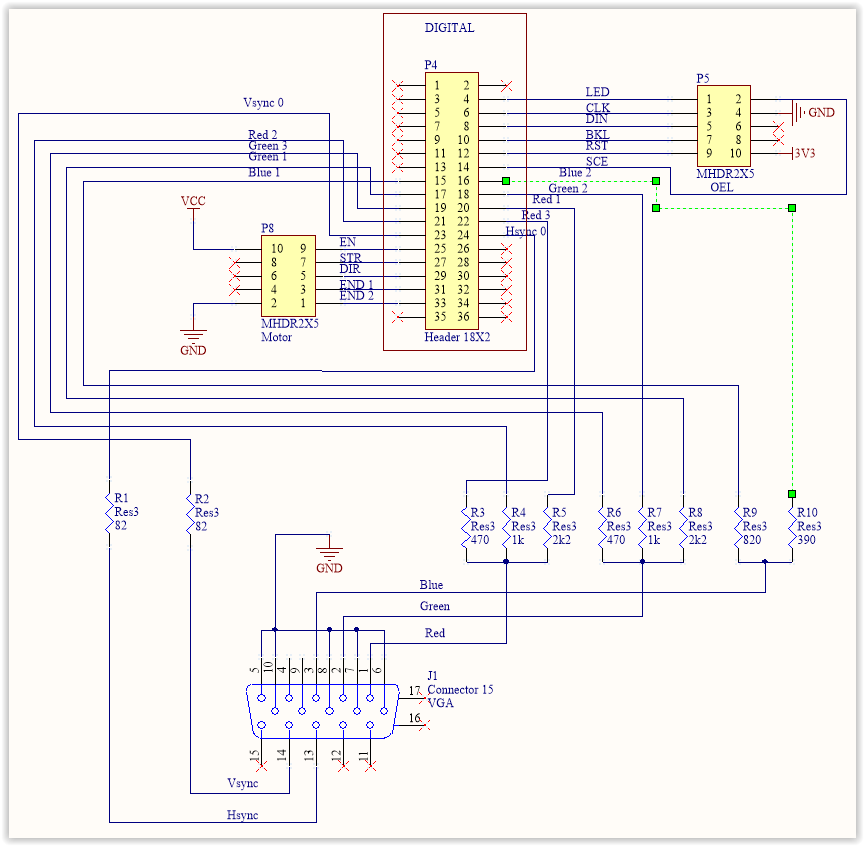
\includegraphics[scale=0.7]{VGA_schm.PNG}
	\caption{Специальная соединительная схема VGA}
	\label{fig:VGASchm}
\end{figure}

\section{Заключение}
Полностью рассмотрена реализуемая аппаратура, полная электрическая схема объединительной платы представлена в приложении А. Готовая электрическая схема позволит уйти от быстро изготовленных и менее надежных монтажных плат (см. рис. \ref{fig:Boards}), которые часто становятся причиной плохих соединений и, как результат, замедляют процесс разработки, ну и конечно, к моменту производства должна быть готова нормальная разводка плат для массового выпуска.

\begin{figure}[ht]
    \centering
    \begin{subfigure}[b]{0.3\textwidth}
    \centering
        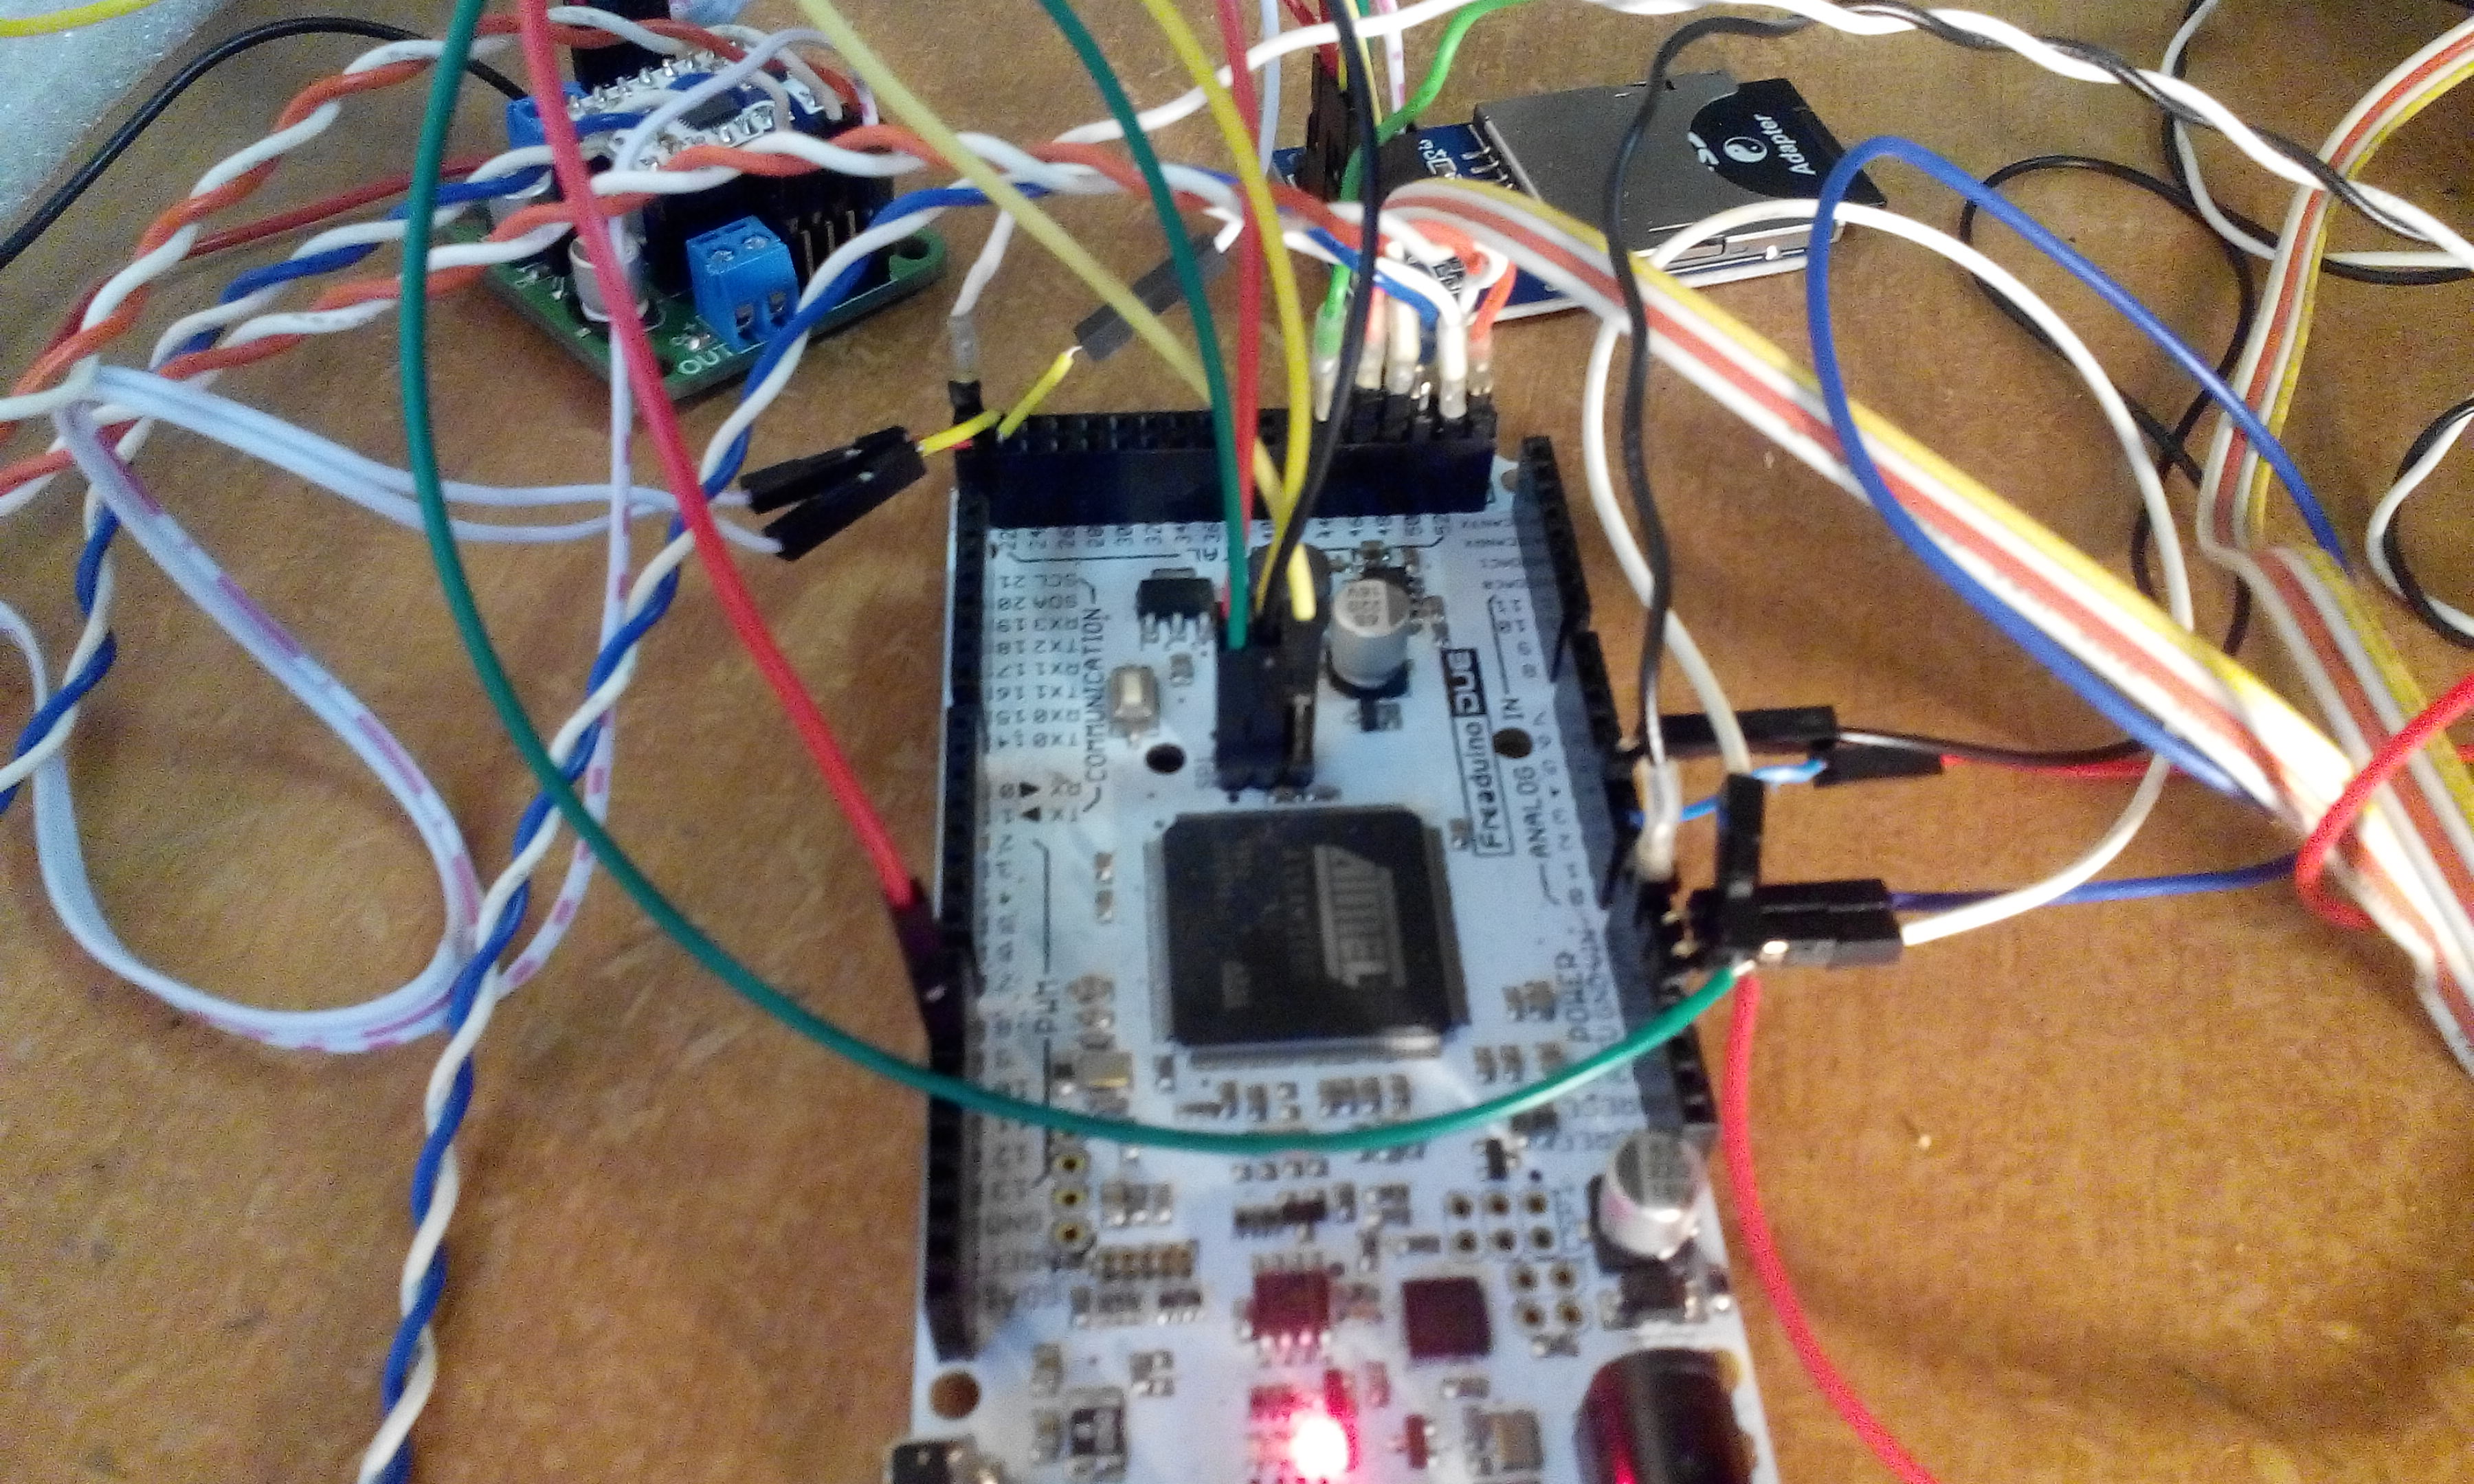
\includegraphics[scale=0.04]{Board1.jpg}
        \caption{}
    \end{subfigure}
    \begin{subfigure}[b]{0.3\textwidth}
    \centering
        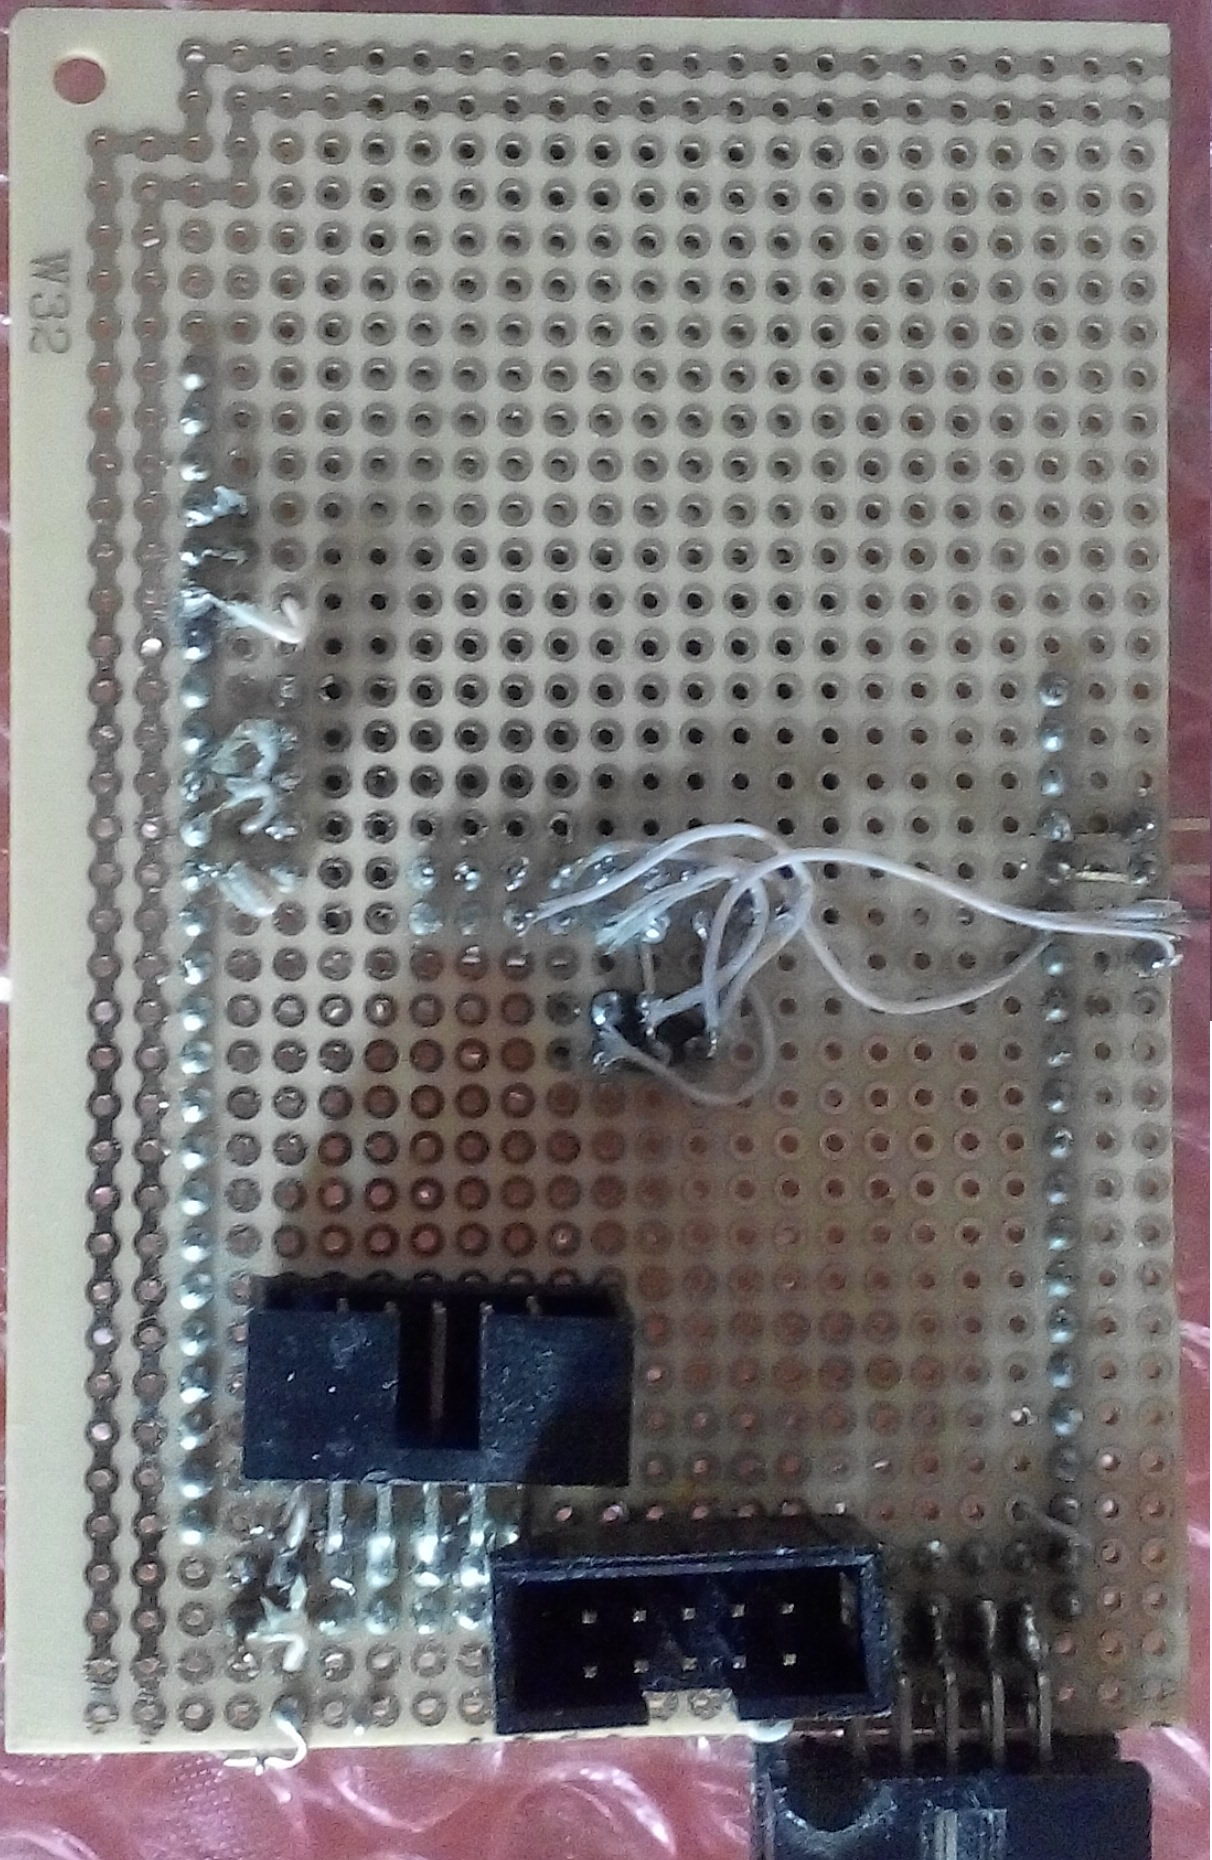
\includegraphics[scale=0.1]{Board2.jpg}
        \caption{}
    \end{subfigure}
    \begin{subfigure}[b]{0.3\textwidth}
    \centering
        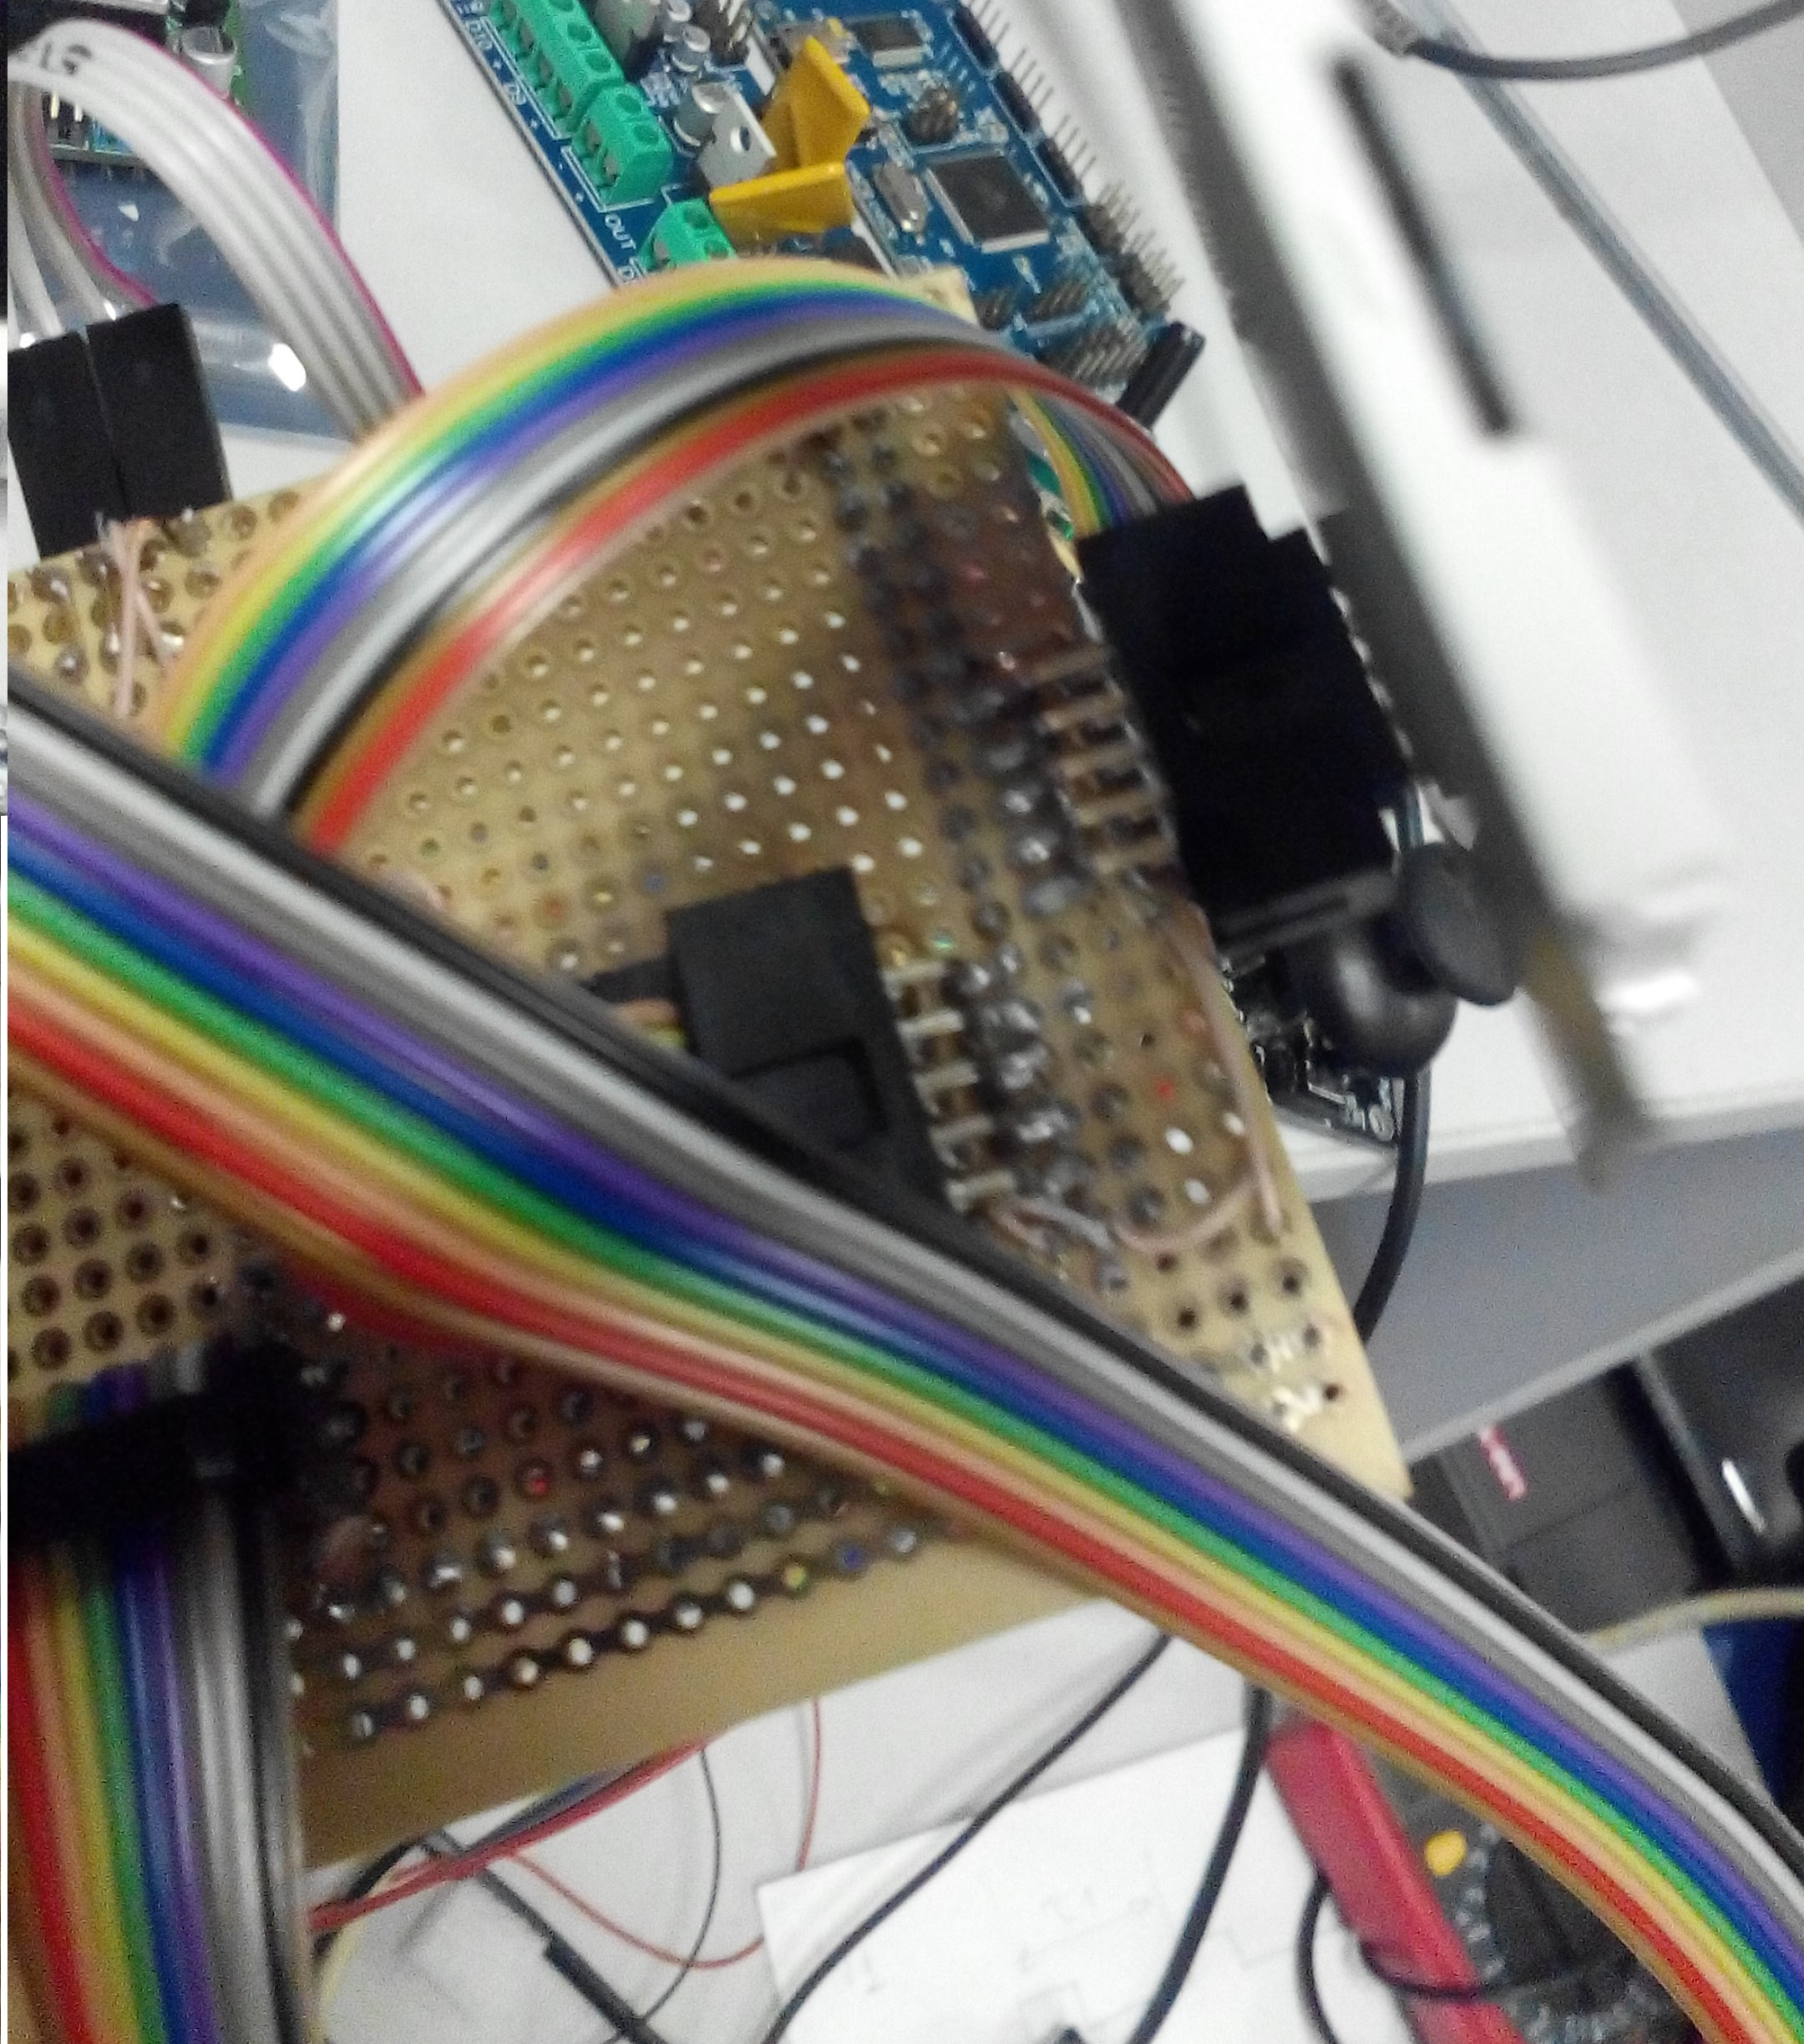
\includegraphics[scale=0.07]{Board3.jpg}
        \caption{}
    \end{subfigure}
    \caption{ (а) - Без объединенной монтажной платы;\\(б) - Объединенная монтажная плата без шин;\\(с) - Объединенная монтажная плата с шинами.}
    \label{fig:Boards}
\end{figure}
В следующей главе рассмотрим реализацию ОС и ее функций.